

\section{Vollständige Induktion}

\begin{framed} 
Sei $P : \N \to \{ \operatorname{falsch}, \operatorname{wahr} \}$. Dann sind die folgenden Bedingungen äquivalent:
  \begin{itemize}
  	\item[(a)] $P(n)$ gilt für alle $n \in \N$.
  	\item[(b)] $P(1)$ gilt, und für alle $n \in \N$ gilt die Implikation $P(n) \Rightarrow P(n+1)$. 
  \end{itemize} 
\end{framed} 

\begin{bem}
Wenn man (a) mit Hilfe von (b) zeigt, so sagt man, dass man die \emph{vollständige Induktion} über $n$ benutzt. Die Aussage $P(1)$ nennt man den \emph{Induktionsanfang}, die Annahme, $P(n)$ sei erfüllt, die \emph{Induktionsvoraussetzung}, und die Herleitung von $P(n+1)$ aus $P(n)$ den \emph{Induktionschritt}. 
\end{bem} 

\begin{bem}
	Auszug aus der Wikipedia\footnote{Artikel zur vollständigen Induktion aus der Wikipedia.}: 
	``
	Die Methode der vollständigen Induktion ist mit dem Dominoeffekt vergleichbar: Wenn der erste Dominostein fällt und durch jeden fallenden Dominostein der nächste umgestoßen wird, wird schließlich jeder Dominostein der unendlich lang gedachten Kette irgendwann umfallen.
	''
	\begin{center} 
	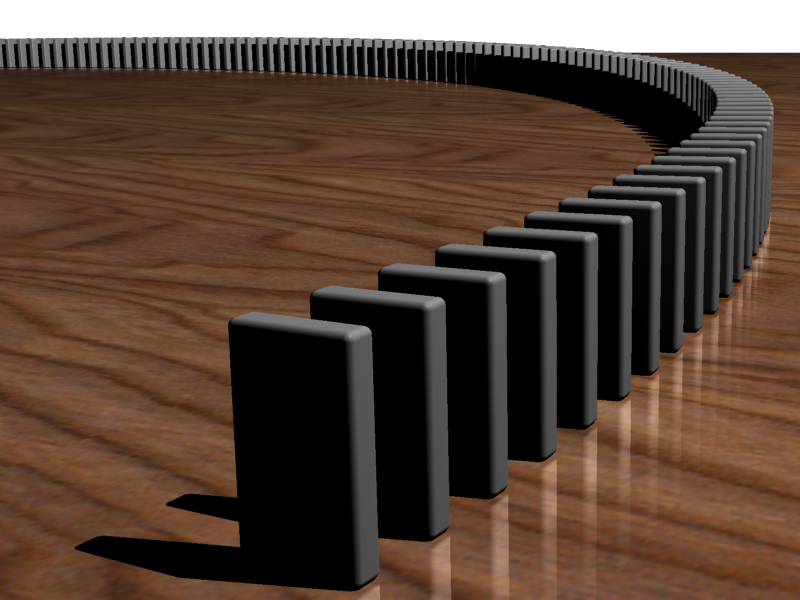
\includegraphics[width=0.5\textwidth]{content/pics/Dominoeffect.png}
	\end{center} 
	\footnote{Bild aus dem Wikipedia-Artikel mathematical induction}
%	/Users/gennnadiyaverkov/Documents/teach/linalg/lineare_algebra_git/contents/pics/Dominoeffect.png
\end{bem} 

Wenn man die Äquivalenz von (a) und (b) für das Prädikat $P(1) \wedge \cdots \wedge P(n)$ an der Stelle von $P(n)$ benutzt, so erhält man, dass (a) auch zur folgenden Behauptung äquivalent ist: 

\begin{itemize}
	\item[(c)] $P(1)$ gilt, und für alle $n \in \N$ gilt die Implikation $P(1) \wedge \cdots \wedge P(n) \Rightarrow P(n+1)$. 
\end{itemize} 

Aussage~(c) ist eine Variante der vollständigen Induktion, mit der Induktionsannahme, $P(k)$ sei für alle $k \in \N$ mit $k \le n$ erfüllt. 

Des Weiteren benutzt man naheliegende Varianten der vollständigen Induktion für Aussagen der Form ``$P(n)$ gilt für alle $n \ge n_0$'' für Prädikate $P : \{ n \in \Z \,:\, n \ge n_0\} \to \{ \operatorname{falsch}, \operatorname{wahr} \}$ und $n_0 \in \Z$. Bei der Induktion in diesem Fall ist die Aussage $P(n_0)$ der Induktionsanfang. 

\begin{bsp}
	Wir zeigen den Existenz-Teil des Fundamentalsatzes der Arithmetik: Jede natürliche Zahl ist Produkt endlich vieler Primzahlen.  Etwas formaler heißt das: jedes $n \in \N$ besitzt die Faktorisierung $\prod_{i=1}^k p_i$ mit $k \in \N_0$, wobei alle $p_i$ in dieser Faktorisierung Primzahlen sind. Wir zeigen die Aussage durch Induktion über $n$. Die Aussage gilt für $n=1$ mit $k=0$ ($1$ ist Produkt von $0$ Primzahlen). Sei $n \in \N$ und man nehme an, allen Zahlen aus $\{1,\ldots,n\}$ lassen sich in endlich viele Primfaktoren zerlegen. Wir betrachten nun die Zahl $n+1$. Ist $n+1$ Primzahl, so ist sie Produkt $n+ 1 = \prod_{i=1}^k p_k$ mit $k=1$ und $p_1=n+1$. Wenn $n+1$ keine Primzahl ist, so existieren $a, b \in \N$ mit $a, b \ge 2$ und $n+1 = ab$. Aus $a,b \ge 2$ und $ab = n+1$ folgt, dass $a$ und $b$ in $\{1,\ldots,n\}$ liegen: denn man hat $a = \frac{n+1}{b} \le \frac{n+1}{2} \le n$, und analog auch $b \le n$. Nach der Induktionsvoraussetzung lassen sich $a$ und $b$ in endlich viele Primfaktoren zerlegen: $a = \prod_{i=1}^s q_i$ mit $b = \prod_{j=1}^t r_j$, wobei $s, t\in \N$ und alle $p_i$ und $r_j$ Primzahlen sind. Dann ist $n+1 = ab = q_1 \cdot \ldots \cdot q_s \cdot r_1 \cdot \ldots \cdot r_t$ Faktorisierung von $n+1$ in $s+t \in \N$ Primfaktoren. 
\end{bsp} 



